\documentclass[11pt]{article}
\usepackage{graphicx, tikz, pgfplots, wrapfig, subcaption}
\usetikzlibrary{calc, intersections, through, backgrounds}
\graphicspath{ {./img/} }
\usepackage[margin=1in]{geometry}
\usepackage{amsfonts, amsmath, amssymb, amsthm, mdframed}
\usepackage[shortlabels]{enumitem}
\newmdtheoremenv{theo}{Theorem}
\usepackage[none]{hyphenat}
\usepackage{fancyhdr}
\usepackage{mathtools}
\newcommand{\equalexpl}[1]{%
    \underset{\substack{\uparrow\\\mathrlap{\text{\hspace{-1em}#1}}}}{=}}

\title{Calculus Chapter 5 Notes}
\author{Qiwen Hua}

\pagestyle{fancy}
\fancyhead{}
\fancyfoot{}
\fancyhead[L]{\slshape \MakeUppercase{Chapter 5 Notes}}
\fancyhead[R]{\slshape Qiwen Hua}
\fancyfoot[C]{\thepage}
\renewcommand{\footrulewidth}{0pt}

\pgfplotsset{compat=1.16}

\begin{document}

\begin{titlepage}
    \begin{center}
        \vspace*{1cm}
        \Large{\textbf{IDS Mathematics}}\\
        %\Large{\textbf{Unit Notes}}\\
        \vfill
        \huge{\textbf{Calculus Chapter 5}}\\[3mm]
        \Large{\textbf{- Integrals -}}\\[1mm]
        \line(1,0){400}\\
        \vfill
        By Qiwen Hua\\
        March 25, 2019
    \end{center}
\end{titlepage}

\setcounter{page}{0}
\tableofcontents
\clearpage

\setcounter{page}{1}
\section{Introduction}
\subsection{Example 1}
\noindent
Consider:\\
Let $ Area=g(x) $, such that: $ \displaystyle{g(x) = \int_{a}^{x}f(x)\ dt} $\\
Considder: let $ f(t) = t $, and $ a=1 $,\\
What is the value of $ g(x) $ when $ x=5 $? i.e. $ g(5)=\ ? $\\
As $x$ changes, then $area$ also changes.
\begin{figure}[h!]
    \begin{subfigure}{0.5\textwidth}
        \centering
        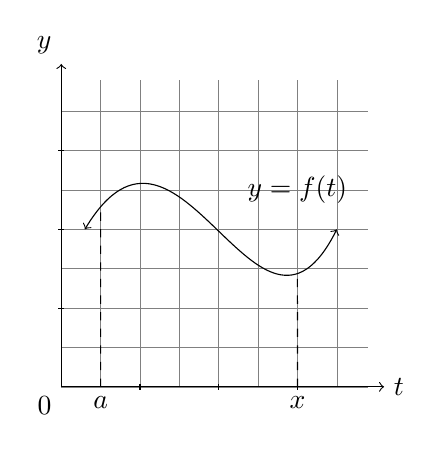
\begin{tikzpicture}[scale=1]
            \draw[step=0.5cm,gray,very thin] (0,0) grid (3.9,3.9);
            \draw[->] (0,0) -- (4.1,0);
            \draw[->] (0,0) -- (0,4.1);
            \node[anchor=south east] at (0,4.1) {$y$};
            \node[anchor=west] at (4.1,0) {$t$};
            \node[anchor=north] at (0.5,0) {$a$};
            \node[anchor=north east] at (0,0) {$0$};
            \foreach \x in {1cm, 2cm, 3cm}
                \draw[] (\x,-1pt) -- (\x,1pt);
            \foreach \y in {1cm, 2cm, 3cm}
                \draw[] (-1pt,\y) -- (1pt,\y);
            \draw[name path=curve][<->] (0.3,2) .. controls (1.5,4) and (2.5,0) .. (3.5,2);
            \path[name path=verta] (3,0) -- (3,4);
            \path[name path=vertb] (0.501,0) -- (0.501,4);
            \draw[name intersections={of=curve and verta, by=x}] [dashed] (3,0) -- (x);
            \draw[name intersections={of=curve and vertb, by=y}] [dashed] (0.501,0) -- (y);
            \node[anchor=north] at (3,0) {$x$};
            \node[] at (3,2.5) {$y=f(t)$};
        \end{tikzpicture}
        \caption[]{Figure 1}
    \end{subfigure}
    \begin{subfigure}{0.5\textwidth}
        \centering
        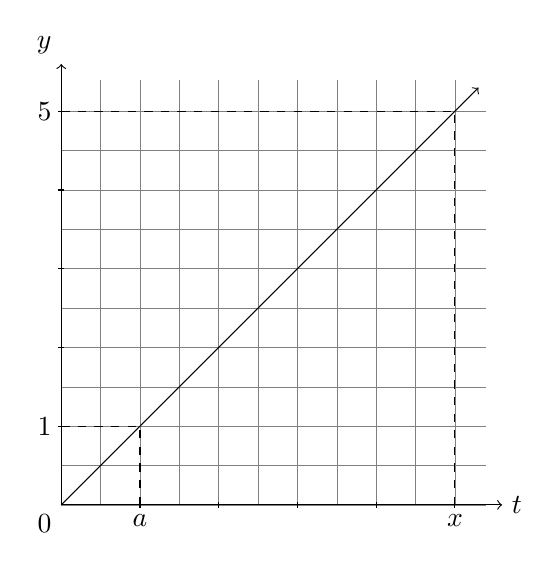
\begin{tikzpicture}[scale=1]
            \draw[step=0.5cm,gray,very thin] (0,0) grid (5.4,5.4);
            \draw[->] (0,0) -- (5.6,0);
            \draw[->] (0,0) -- (0,5.6);
            \node[anchor=south east] at (0,5.6) {$y$};
            \node[anchor=west] at (5.6,0) {$t$};
            \node[anchor=north east] at (0,0) {$0$};
            \node[anchor=north] at (1,0) {$a$};
            \node[anchor=north] at (5,0) {$x$};
            \foreach \x in {1cm, 2cm, 3cm, 4cm, 5cm}
                \draw[] (\x,-1pt) -- (\x,1pt);
            \foreach \y in {1cm, 2cm, 3cm, 4cm, 5cm}
                \draw[] (-1pt,\y) -- (1pt,\y);
            \draw[->] (0,0) -- (5.3,5.3);
            \node[anchor=east] at (0,1) {$1$};
            \node[anchor=east] at (0,5) {$5$};
            \draw[dashed] (1,0) -- (1,1);
            \draw[dashed] (5,0) -- (5,5);
            \draw[dashed] (0,1) -- (1,1);
            \draw[dashed] (0,5) -- (5,5);
        \end{tikzpicture}
        \caption{Figure 2}
    \end{subfigure}
\end{figure}

In $Figure\ 2$ we know: $\displaystyle{g(x)=\int_{a}^{x}f(t)\ dt}$\\
\begin{align*}
    g(5)&=\int_{1}^{5}f(t)\ dt=\int_{0}^{5}f(t)\ dt-\int_{0}^{1}f(t)\ dt\\
    &=\frac{(5)(5)}{2}-\frac{(1)(1)}{2}\\
    &=\frac{25}{2}-\frac{1}{2}=12
\end{align*}

\textbf{GENERAL CASE}: \[
    g(x)=\int_{a}^{x}f(t)\ dt=\int_{0}^{x}f(t)\ dt-\int_{0}^{a}f(t)\ dt
\]

Recall:
\begin{align*}
    \int_{0}^{4}(x^3-6x)dx&=\frac{1}{4}x^4-\frac{6}{2}x^2\ \bigg]_0^4\\
    &=\Big(\frac{1}{4}(4)^4-3(4)^2\Big)-\Big(\frac{1}{4}(0)^4-3(0)^2\Big)\\
    &=4^3-3\cdot4^2=16
\end{align*}

\pagebreak
\subsection{Example 2}
Let $f(x)=x^3$. Find area from $x=0 \text{ to } x=1$ using the Riemann Sum definition.
\begin{figure}[h]
    \centering
    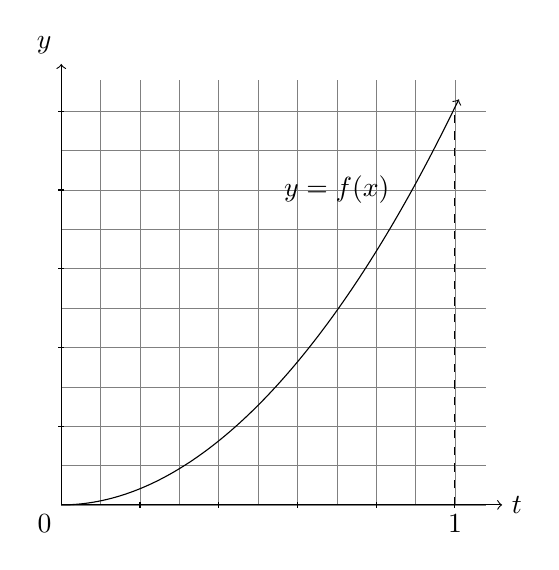
\begin{tikzpicture}[scale=1]
        \draw[step=0.5cm,gray,very thin] (0,0) grid (5.4,5.4);
        \draw[->] (0,0) -- (5.6,0);
        \draw[->] (0,0) -- (0,5.6);
        \node[anchor=south east] at (0,5.6) {$y$};
        \node[anchor=west] at (5.6,0) {$t$};
        \node[anchor=north east] at (0,0) {$0$};
        \node[anchor=north] at (5,0) {$1$};
        \foreach \x in {1cm, 2cm, 3cm, 4cm, 5cm}
            \draw[] (\x,-1pt) -- (\x,1pt);
        \foreach \y in {1cm, 2cm, 3cm, 4cm, 5cm}
            \draw[] (-1pt,\y) -- (1pt,\y);
        \draw[->] (0,0) parabola (5.05,5.1515);
        \draw[dashed] (5,0) -- (5,5);
        \node[] at (3.5,4) {$y=f(x)$};
    \end{tikzpicture}
    \caption{Example 2}
\end{figure}

\begin{align*}
    \text{We know: }\int_{a}^{b}f(x)dx&=\lim_{n\to\infty}\sum_{i=1}^{n}f(x^*)\Delta x\\
    \text{Also: }\int_{a}^{b}f(x)dx&=\int_{0}^{b}f(x)dx-\int_{0}^{a}f(x)dx\\
    \therefore \int_{2}^{4}f(x)dx&=\int_{0}^{4}f(x)dx-\int_{0}^{2}f(x)dx\\
    &=\lim_{n\to\infty}\sum_{i=1}^{n}f(x_i)\Delta x - \lim_{n\to\infty}\sum_{i=1}^{n}f(x_i)\Delta x\\
    &=\lim_{n\to\infty}\Big[\sum_{i=1}^{n}\Big(\frac{4}{n}i^3\Big)\cdot \frac{4}{n}\Big]-\lim_{n\to\infty}\Big[\sum_{i=1}^{n}\Big(\frac{2}{n}i^3\Big)\cdot \frac{2}{n}\Big]
\end{align*}

\pagebreak
\subsection{}
\begin{theo}
    \[
        \int_{a}^{b}[f(x)+g(x)]dx=\int_{a}^{b}f(x)dx+\int_{a}^{b}g(x)dx
    \]
\end{theo}
\begin{proof}
    We know:
    \begin{align*}
        \int_{a}^{b}(f(x)+g(x))&=\lim_{n\to\infty}\sum_{i=1}^{n}(f(x_i^*)+g(x_i^*))\Delta x\\
        &=\lim_{n\to\infty}\Big\{\Delta x \cdot \sum_{i=1}^{n}[f(x_i^*)+g(x_i^*)]\Big\}\\
        &=\lim_{n\to\infty}\Big[\sum_{i=1}^{n}f(x_i^*)\Delta x+\sum_{i=1}^{n}g(x_i^*)\Delta x\Big]\\
        &=\lim_{n\to\infty}\Big[\sum_{i=1}^{n}f(x_i^*)\Delta x\Big]+\lim_{n\to\infty}\Big[\sum_{i=i}^{n}g(x_i^*)\Delta x\Big]\\
        &=\int_{a}^{b}f(x)dx+\int_{a}^{b}g(x)dx
    \end{align*}
\end{proof}
\subsubsection{Example 2}
Solve: $\displaystyle{\int_{0}^{3}(x^3-6x)dx}$ (using properties of integral).
\begin{align*}
    \int_{0}^{3}(x^3-6x)dx &= \int_{0}^{3}x^3\ dx - 6\int_{0}^{3}x\ dx\\
    &= \lim_{n\to\infty}\sum_{i=1}^{n}(x_i)^3\cdot \frac{3}{n} - 6\cdot \frac{9}{2}\\
    &= -\frac{27}{4}
\end{align*}

\subsubsection{Example 6}
Use the properties of integrals to evaluate $\displaystyle{\int_{0}^{1}(4+3x^2)\ dx}$.
\begin{align*}
    \text{We know: }\int_{0}^{1}x^2\ dx &= \lim_{n\to\infty}\sum_{i=1}^{n}(x^*)^2\Delta x\\
    &=\lim_{n\to\infty}\sum_{i=1}^{n}\Big(\frac{i}{n}\Big)^2\frac{1}{n} = \frac{1}{3}\\
    \text{And: }\int_{0}^{1}(4+3x^2)\ dx &= \int_{0}^{1}4\ dx + \int_{0}^{1}x^2\ dx\\
    &= 4(1-0) +3(\frac{1}{3})
\end{align*}

\subsubsection{Example 8}
It is know that $\displaystyle{\int_{0}^{10}f(x)dx=17 \text{ and }\int_{0}^{8}f(x)dx=12}$. Find $\displaystyle{\int_{8}^{10}f(x)dx}$.
\begin{align*}
    \int_{8}^{10}f(x)dx &= \int_{0}^{10}f(x)dx - \int_{0}^{8}f(x)dx\\
    &= 17-12 = 5
\end{align*}

\section{Anti-derivatives}
\subsection{Introduction}
Consider the function $f(t)=t$:
\begin{enumerate}
    \item $ \displaystyle{g(x)=\int_{a}^{x}f(t)dt} $
    \item $ \displaystyle{g'(x) = \frac{d}{dx}\int_{a}^{x}t\ dt=x} $
\end{enumerate}
Supports that \textbf{differentiate} is the \textbf{inverse proceedure} to \textbf{integration} (connects to \textbf{anti-derivative}).
\\[10pt]
\noindent
Now... Suppose $f(t)=t$. let $a=0 \text{. Find }g(x)$.
\begin{figure}[h]
    \begin{subfigure}{0.5\textwidth}
        \centering
        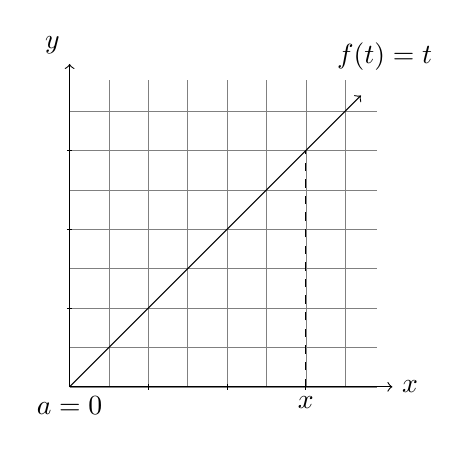
\begin{tikzpicture}[scale=1]
            \draw[step=0.5cm,gray,very thin] (0,0) grid (3.9,3.9);
            \draw[->] (0,0) -- (4.1,0);
            \draw[->] (0,0) -- (0,4.1);
            \node[anchor=south east] at (0,4.1) {$ y $};
            \node[anchor=west] at (4.1,0) {$ x $};
            \foreach \x in {1cm, 2cm, 3cm}
                \draw[] (\x,-1pt) -- (\x,1pt);
            \foreach \y in {1cm, 2cm, 3cm}
            \draw[] (-1pt,\y) -- (1pt,\y);
            \draw[->] (0,0) -- (3.7,3.7);
            \draw[dashed] (3,0) -- (3,3);
            \node[anchor=north] at (0,0) {$a=0$};
            \node[] at (4,4.2) {$f(t)=t$};
            \node[anchor=north] at (3,0) {$x$};
        \end{tikzpicture}
        \caption{$f(t)=t$}
        \label{a}
    \end{subfigure}
    \begin{subfigure}{0.5\textwidth}
        \centering
        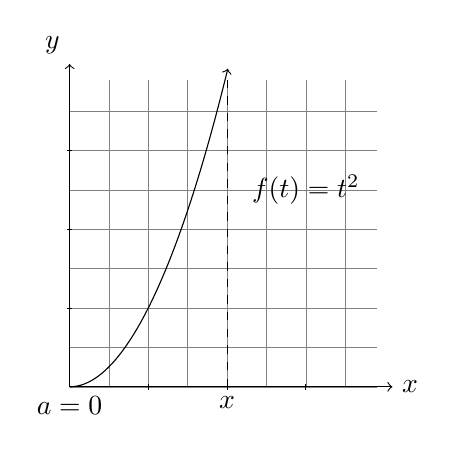
\begin{tikzpicture}[scale=1]
            \draw[step=0.5cm,gray,very thin] (0,0) grid (3.9,3.9);
            \draw[->] (0,0) -- (4.1,0);
            \draw[->] (0,0) -- (0,4.1);
            \node[anchor=south east] at (0,4.1) {$ y $};
            \node[anchor=west] at (4.1,0) {$ x $};
            \node[anchor=north] at (0,0) {$ a=0 $};
            \foreach \x in {1cm, 2cm, 3cm}
                \draw[] (\x,-1pt) -- (\x,1pt);
            \foreach \y in {1cm, 2cm, 3cm}
            \draw[] (-1pt,\y) -- (1pt,\y);
            \draw[->] (0,0) parabola (2.01,4.04);
            \node[] at (3,2.5) {$f(t)=t^2$};
            \draw[dashed] (2,0) -- (2,4);
            \node[anchor=north] at (2,0) {$x$};
        \end{tikzpicture}
        \caption{$f(t)=t^2$}
        \label{b}
    \end{subfigure}
\end{figure}

\noindent
In Figure (a), $ \displaystyle{g(x) = \int_{0}^{x}t\ dt = \frac{1}{2}x^2} \ (*)$, from geometry.\\
Suppose we want $ g'(x) $.
From $ (*) $, $ \displaystyle{g'(x)=\frac{d}{dx}\int_{0}^{x}t\ dt=\frac{d}{dx}\Big(\frac{1}{2}x^2\Big)} $.\\
$\therefore \displaystyle{g'(x)=\frac{d}{dx}\int_{0}^{x}t\ dt=x} $.
\\[12pt]
\noindent
Consider Figure (b):
\begin{align*}
    \int_{0}^{x}t^2\ dx
    &= \lim_{n\to\infty}\Big[\sum_{i=1}^{n}\Big(\frac{xi}{n}\Big)^2\cdot\frac{x}{n}\Big]\\
    &= \lim_{n\to\infty}\frac{x}{n}\sum_{i=1}^{n}\Big(\frac{xi}{n}\Big)^2\\
    &= \lim_{n\to\infty}\Big(\frac{x}{n}\Big)^3 \sum_{i=1}^{n}i^2\\
    &= \lim_{n\to\infty}\Big(\frac{x}{n}\Big)^3\cdot \frac{n(n+1)(2n+1)}{6}\\
    &= x^3 \cdot \lim_{n\to\infty}\frac{(n+1)(2n+1)}{6n^2}\\
    &= \frac{1}{3}x^3\\
\end{align*}
$\text{Therefore: } \displaystyle{g(x)=\int_{0}^{x}t^2\ dx=\frac{1}{3}x^3 \text{ (*)}}$\\[3pt]
$ Area \Rightarrow \displaystyle{g(x) = \int_{0}^{x}t^2\ dt} $
From (*): $ \displaystyle{g'(x)=\frac{d}{dx}\int_{0}^{x}t^2\ dx=x^2} $.

\section{The Foundamental Theorem of Calculus Part 1}
\begin{theo}
    If $ f $ is continuous on $ [a,b] $, then the function $ g $ defined by: $ g(x) = \int_{a}^{x}f(t)\ dt,\ a\leq x\leq b $, is continuous on $ [a,b] $, and differentiable on $ (a,b) $, and $ g'(x)=f(x) $.
\end{theo}
\subsection{Example 2}
Find the derivative of $ \displaystyle{g(x)=\int_{0}^{x}\sqrt{1+t^2}\ dt} $.
\[
    g'(x)=\frac{d}{dx}\int_{0}^{x}\sqrt{1+t^2}\ dt\equalexpl{FTC Part 1} \sqrt{1+t^2}
\]

\subsection{Example 4 - p.g 384}
Find $ \displaystyle{\frac{d}{dx}\int_{1}^{x^4}\sec t\ dt} $.
\begin{align*}
    \text{let }g(x)&=\int_{1}^{x^4}\sec t\ dt\\
    g'(x) &= \frac{d}{dx}\int_{1}^{x^4}\sec t\ dt \equalexpl{let $ u=x^4 $} \frac{d}{dx}\int_{1}^{u}\sec t\ dt\\
    &\equalexpl{chain rule} \frac{d}{du}\Big(\int_{1}^{u}\sec t\ dt \Big)\frac{du}{dx}\\
    &= \sec u \cdot \frac{d}{dx}(u) = \sec(x^4)\cdot 4x^3\\
    g'(x) &= \frac{d}{dx}\int_{1}^{x^4}=\sec(x)^4\cdot (4x^3)\\
    &= 4x^3\cdot \sec(x^4)
\end{align*}

Suppose: $ \displaystyle{\frac{d}{dx}\int_{x^2}^{x^4}\sec t\ dt} $.
\begin{figure}[h]
    \centering
        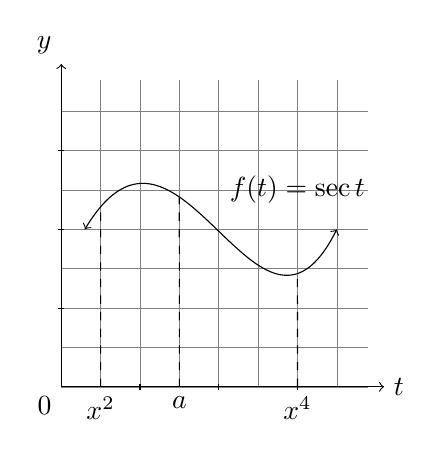
\begin{tikzpicture}[scale=1]
            \draw[step=0.5cm,gray,very thin] (0,0) grid (3.9,3.9);
            \draw[->] (0,0) -- (4.1,0);
            \draw[->] (0,0) -- (0,4.1);
            \node[anchor=south east] at (0,4.1) {$y$};
            \node[anchor=west] at (4.1,0) {$t$};
            \node[anchor=north] at (0.5,0) {$x^2$};
            \node[anchor=north] at (3,0) {$x^4$};
            \node[anchor=north] at (1.5,0) {$a$};
            \node[anchor=north east] at (0,0) {$0$};
            \foreach \x in {1cm, 2cm, 3cm}
                \draw[] (\x,-1pt) -- (\x,1pt);
            \foreach \y in {1cm, 2cm, 3cm}
                \draw[] (-1pt,\y) -- (1pt,\y);
            \draw[name path=curve][<->] (0.3,2) .. controls (1.5,4) and (2.5,0) .. (3.5,2);
            \path[name path=verta] (3,0) -- (3,4);
            \path[name path=vertb] (0.501,0) -- (0.501,4);
            \path[name path=vertc] (1.5,0) -- (1.5,4);
            \draw[name intersections={of=curve and verta, by=x}] [dashed] (3,0) -- (x);
            \draw[name intersections={of=curve and vertb, by=y}] [dashed] (0.501,0) -- (y);
            \draw[name intersections={of=curve and vertc, by=z}] [dashed] (1.5,0) -- (z);
            \node[] at (3,2.5) {$f(t)=\sec t$};
        \end{tikzpicture}
\end{figure}
\begin{align*}
    \text{We know: } \int_{x^2}^{x^4}\sec t\ dt &= \int_{x^2}^{a}\sec t\ dt + \int_{a}^{x^4}\sec t\ dt\\
    \text{And: }\int_{x^2}^{a}\sec t\ dt &= -\int_{a}^{x^2}\sec t\ dt\\
    \therefore \int_{x^2}^{x^4}\sec t\ dt &= \int_{a}^{x^4}\sec t\ dt - \int_{a}^{x^2}\sec t\ dt
\end{align*}

\pagebreak
\section{The Foundamental Theorem of Calculus Part 2}
\begin{theo}
    If $ f $ is continuous on $ [a,b] $, then $ \displaystyle{\int_{a}^{b}f(x)\ dx=F(b) - F(a)} $, where $ F $ is any\\[2pt] antiderivative of $ f $, that is, a function such that $ F' = f $.
\end{theo}
\subsection{Indefinite Integral}
\subsubsection{Example 1}
Find $ \displaystyle{\int(10x^4-2\sec ^2x)\ dx} $.
\begin{align*}
    \int(10x^4-2\sec ^2x)\ dx
    &= \frac{10}{4+1}x^{4+1}-s\tan x+C\\
    &= 2x^5-2\tan x+C
\end{align*}

\subsubsection{Example 2}
Evaluate $ \displaystyle{\int \frac{\cos \theta}{\sin ^2 \theta}\ d\theta} $.
\begin{align*}
    \int \frac{\cos \theta}{\sin ^2 \theta}\ d\theta
    &= \int \Big(\frac{\cos \theta}{\sin \theta}\cdot \frac{1}{\sin \theta} \Big)\  d\theta\\
    &= \int \cot \theta \cdot \csc \theta \cdot d \theta\\
    \therefore \int \frac{\cos \theta}{\sin ^2 \theta}d \theta &= -\csc \theta + C
\end{align*}

\subsubsection{Example 3}
Evaluate $ \displaystyle{\int_{0}^{3}(x^3-6x)\ dx} $.
\begin{align*}
    \int_{0}^{3}(x^3-6x)\ dx
    &= \frac{1}{4}x^4-3x^2 \bigg]_0^3\\
    &= \Big[ \frac{1}{4}(x)^4 - 3(3)^2 \Big] - 0\\
    &= -6.75
\end{align*}

\subsubsection{Example 4}
Evaluate $ \displaystyle{\int_{0}^{2}\Big(2x^3-6x+\frac{3}{x^2+1}\Big)\ dx} $.
\begin{align*}
    \int_{0}^{2}\Big(2x^3-6x+\frac{3}{x^2+1}\Big)\ dx
    &= \frac{2}{4}x^4 - \frac{6}{2}x^2 + 3 \arctan x \bigg]_0^2\\
    &= \frac{1}{2}(x)^4 - 3(x)^2 + 3\arctan 2 - 0\\
    &= -4 + 3\arctan 2
\end{align*}

\subsubsection{Example 5}
Evaluate $ \displaystyle{\int_{0}^{2}\frac{2t^2+t^2\sqrt{t} - 1}{t^2}\ dt} $.
\begin{align*}
    \int_{1}^{9}\frac{2t^2+t^2\sqrt{t} - 1}{t^2}\ dt
    &= \int_{1}^{9}(2+t^{1/2} - t^{-2})\ dt\\
    &= 2t + \frac{t^{3/ 2}}{\frac{3}{2}-\frac{t^{-1}}{-1}}\Bigg]_1^9\\
    &= \Big(2\cdot 9 + \frac{2}{3}\cdot 9^{3/ 2}+\frac{1}{9}\Big)-\Big(2\cdot1 + \frac{2}{3}\cdot 1^{3/2}+1\Big)\\
    &=32 \frac{4}{9}
\end{align*}

\subsubsection{Example 6}
A particle moves alopng a line so that its velocity at time $ t $ is $ v(t)=t^2-t-6 $.
\begin{enumerate}[a)]
    \item Find the displacement of the particle during the time period $ 1\leq t\leq 4 $.
    \item Find the distance traveled during this time period.
\end{enumerate}

\noindent
a)
\begin{align*}
    S(4)-S(1) &= \int_{1}^{4}v(t)\ dt = \int_{1}^{4}(t^2-t-6)\ dt\\
    &= \bigg[ \frac{t^3}{3} - \frac{t^2}{2} - 6t \bigg]_1^4 = -\frac{9}{2}\\
\end{align*}
b) Note that $ v(t)=t^2-t-6=(t-3)(t+2) $ and so $ v(t)\leq 0 $ on the interval $ [1,3] $ and $ v(t)\geq 0 \text{ on } [3,4] $. Thus, the distance traveled is
\begin{align*}
    \int_{1}^{4}|v(t)|
    &= \int_{1}^{3}[-v(t)]dt + \int_{3}^{4}v(t)dt\\
    &= \int_{1}^{3}(-t^2+t+6)dt + \int_{3}^{4}(t^2-t-6)dt\\
    &= \bigg[ -\frac{t^3}{3} + \frac{t^2}{2} + 6t\bigg]_1^3 + \bigg[\frac{t^3}{3} - \frac{t^2}{2} - 6t\bigg]_3^4\\
    &= \frac{61}{6}
\end{align*}

\pagebreak
\section{The Substitution Rule}
\begin{theo}
    If $ u=g(x) $ is a differentiable function whose range is an interval $ I $ and $ f $ is continuous on $ I $, then \[
        \int f(g(x))g'(x)dx = \int f(u) du
    \]
\end{theo}
\subsection{Example 1}
Find $ \displaystyle{\int[x^3\cos (x^4+2)]dx} $.
\\[8pt]
We make the substitution $ u=x^4+2 $ because its differential is $ du = 4x^3\ dx $, which occurs in the integral. Thus using $ x^3\ dx=dy/4 $ and the Substitution Rule, we have
\begin{align*}
    \int x^3\cos(x^4+2)dx &= \int \cos u \cdot \frac{1}{4}\ du = \frac{1}{4} \int \cos u\ du\\
    &=\frac{1}{4}\sin u + C\\
    &= \frac{1}{4}\sin (x^4+2) +C
\end{align*}

\subsection{Example 2}
Evaluate $ \displaystyle{\int \sqrt{2x+1}\ dx} $.
\\[8pt]
Let $ u=2x+1 $. Then $ du=2\ dx $, so $ dx=du/2 $. Thus the Substitution Rule gives
\begin{align*}
    \int \sqrt{2x+1}\ dx
    &= \int \sqrt{u}\ \frac{du}{2} = \frac{1}{2}\int u^{1/2}du\\
    &= \frac{1}{2}\cdot \frac{u^{3/2}}{3/2} + C = \frac{1}{3}u^{3/2} +C\\
    &= \frac{1}{3}(2x+1)^{3/2} +C
\end{align*}

\subsection{Example 3}
Evaluate $ \displaystyle{\int \frac{x}{\sqrt{1-4x^2}}\ dx} $.
\\[8pt]
Let $ u=1-4x^2 $. THne $ du=-8x\ dx $, so $ x\ dx = -\frac{1}{8}du $ and
\begin{align*}
    \int \frac{x}{\sqrt{1-rx^2}}\ dx &= -\frac{1}{8}\int \frac{1}{\sqrt{u}}\ du = -\frac{1}{8}\int u^{1/2}\ du\\
    &= -\frac{1}{8}(x\sqrt{u}) + C = -\frac{1}{4}\sqrt{1-4x^2} + C
\end{align*}

\pagebreak
\subsection{Example 4}
Evaluate $ \displaystyle{\int e^{5x}\ dx} $.
\\[8pt]
Let $ u=5x $, then $ du=5\ dx $, so $ dx = \frac{1}{5}du $. Therefore
\begin{align*}
    \int e^{5x} &= \frac{1}{5}\int e^u \ du = \frac{1}{5}e^u + C = \frac{1}{5}e^{5x} + C
\end{align*}

\subsection{Example 5}
Evaluate $ \displaystyle{\int \sqrt{1+x^2}\ x^5\ dx} $.
\\[8pt]
An Appropriate substitution ecomes more obvious if we factor $ x^5 $ as $ x^4 \cdot x $. Let $ u = 1+x^2 $. Then $ du = 2x\ dx $, so $ x\ dx = du/2 $. Also $ x^2 = u - 1 $, so $ x^4 = (u-1)^2 $:
\begin{align*}
    \int \sqrt{1+x^2}x^5\ dx
    &= \int \sqrt{1+x^2}x^4\cdot x\ dx\\
    &= \int \sqrt{u} (u-1)^2\ \frac{du}{2}
    =  \frac{1}{2}\int \sqrt{u}(u^2 - 2u +1)\ du\\
    &= \frac{1}{2}\int (u^{5/2} - 2u^{3/2} + u^{1/2})\ du\\
    &= \frac{1}{2}(\frac{2}{7}u^{7/2} - 2\cdot \frac{2}{5}u^{5/2} + \frac{2}{3}u^{3/2}) + C\\
    &= \frac{1}{7}(1+x^2)^{7/2} - \frac{2}{5}(1+x^2)^{5/2} + \frac{1}{3}(1+x^2)^{3/2} + C
\end{align*}

\subsection{Example 6}
Evaluate $ \displaystyle{\int \tan x\ dx} $.
\\[8pt]
First we write tangent in terms of since and cosine:\[
    \int \tan x\ dx = \int \frac{\sin x}{\cos x}\ dx
\]
This suggests that we should substitute $ u = \cos x $, since then $ du = -\sin x\ dx $ and so $ \sin x\ dx = -du $:
\begin{align*}
    \int \tan x\ dx
    &= \int \frac{\sin x }{\cos x}\ dx = -\int \frac{du}{u}\\
    &= -\ln |u| + C = -\ln|\cos x| + C
\end{align*}

\pagebreak
\subsection{Definite Integrals}
\begin{theo}[\textbf{The Substitution Rule For Definite Integrals}]
    If $ g' $ is continuous on $ [a,b] $ and $ f $ is continuous on the range of $ u=g(x) $, then \[
        \int_{a}^{b}f(g(x))g'(x)\ dx = \int_{g(a)}^{g(b)}f(u)\ du
    \]
\end{theo}
Consider: $ \displaystyle{\int_{0}^{4}\sqrt{2x+1}\ dx} $.\\
\textbf{\textit{Method 1: }}For Now, consider the indefinite integral for $ \displaystyle{\int \sqrt{2x+1}} $:
\\[8pt]
Let $ u = 2x+1 $. Then $ du = 2\ dx $ and $ dx = \frac{du}{2} $. Therefore
\begin{align*}
    \int \sqrt{2x+1}\ dx
    &= \int \sqrt{u} \cdot \frac{du}{2}\\
    &= \frac{1}{2}\int u^{1/2}\ du\\
    &= \frac{1}{2}\Big[ \Big(\frac{1}{1/2} + 1\Big)\ u^{1/2 + 1} \Big] + C\\
    &= \frac{1}{2} \cdot \frac{2}{3}u^{3/2} + C\\
    &= \frac{1}{3}(2x+1)^{3/2} + C
\end{align*}
Now:
\begin{align*}
    \int_{0}^{4}\sqrt{2x+1}\ dx
    &= \frac{1}{3}(2x+1)^{3/2} \bigg]_0^4\\
    &= \frac{1}{3}[(2)(4)+1]^{3/2} - \frac{1}{3}[(2)(0)+1]^{3/2}\\
    &= \frac{26}{3}
\end{align*}
\textbf{\textit{Method 2: }} For Now, consider the indefinite integral for $ \displaystyle{\int \sqrt{2x+1}} $:
\\[8pt]
Let $ u=2x+1 $. When $ x=4\text{ , } u=9 \text{ and when } x=0\text{ , } u = 1 $.
\begin{align*}
    \int_{0}^{4}\sqrt{2x+1}
    &= \int_{1}^{9}\frac{1}{2}\sqrt{u}\ du
    =  \frac{1}{2} \cdot \frac{2}{3}u^{3/2} \bigg]_1^9\\
    &= \frac{1}{3}(9^{3/2} - 1^{3/2}) = \frac{26}{3}
\end{align*}

\subsection{Example 8}
Evaluate $ \displaystyle{\int_{1}^{2}\frac{dx}{(3-5x)^2}} $.
\\[8pt]
Let $ u=3-5x $. Then $ du = -5\ dx $, so $ dx = -du/5 $. When $ x = 1 \text{, } u = -2 \text{ and when, } x=2, u=-7 $. Thus
\begin{align*}
    \int_{1}^{2}\frac{dx}{(3-5x)^2}
    &= -\frac{1}{5}\int_{-2}^{-7}\frac{du}{u^2}\\
    &= -\frac{1}{5}\bigg[ -\frac{1}{u}\bigg]_{-2}^{-7} = \frac{1}{5u}\bigg]_{-2}^{-7}\\
    &= -\frac{1}{5}\bigg(-\frac{1}{7}+\frac{1}{2}\bigg) = \frac{1}{14}
\end{align*}

\subsection{Example 9}
Evaluate $ \displaystyle{\int_{1}^{e}\frac{\ln x}{x}\ dx} $.
\\[8pt]
Let $ u=\ln x $. Then $ du=\frac{dx}{x} $. When $ x=1\text{ , }u=|\ln x|=0\text{ and when }x=e\text{ , }u=\ln e=1 $.
\[
    \therefore \int_{1}^{e}\frac{\ln x}{x}\ dx = \int_{0}^{1}u\ du = \frac{u^2}{2}\bigg]_0^1 = \frac{1}{2}
\]
\\[20pt]
\begin{theo}[\textbf{Integrals of Symmetric Functions} ]
    Suppose $ f $ is continuous on $ [a,-a] $.
    \begin{enumerate}[a)]
        \item If $ f $ is even $ [f(-x)] = f(x) $, then $ \int_{-a}^{a}f(x)\ dx = 2 \int_{0}^{a}f(x)\ dx $.
        \item If $ f $ is odd $ [f(-x)] = -f(x) $, then $ \int_{-a}^{a}f(x)\ dx = 0 $.
    \end{enumerate}
\end{theo}
\subsection{Example 10}
Evaluate $ \displaystyle{\int_{-2}^{2}(x^6+1)\ dx} $.\\
\begin{figure}[h]
    \centering
    \begin{tikzpicture}[scale=0.6]
        \begin{axis}[
            axis y line=middle,
            axis x line=middle]
            \addplot[<->][
                color=black,
                domain=-5:5,
                samples=100
            ]{x^6+1};
        \end{axis}
    \end{tikzpicture}
    \caption{$ f(x)=x^6+1 $}
    \label{Label}
\end{figure}

\noindent
Since $ f(x)=x^6+1 $ satisfies $ f(-x)=f(x) $. it is even and so
\begin{align*}
    \int_{-2}^{2}(x^6+1)\ dx
    &= 2\ \int_{0}^{2}(x^6+1)\ dx\\
    &= 2\bigg[ \frac{1}{7}x^7 + x\bigg]_0^2
    =  2\bigg(\frac{128}{7}+2\bigg)
    =  \frac{284}{7}
\end{align*}

\subsection{Example 11}
Evaluate $ \displaystyle{\int_{-1}^{1}\frac{\tan x}{1+x^2+x^4}\ dx} $.\\
\begin{figure}[h]
    \centering
    \begin{tikzpicture}[scale=0.8]
        \begin{axis}[
            axis y line=middle,
            axis x line=middle
        ]
            \addplot[<->][
                color=black,
                domain=-5:5,
                samples=900
            ]{(tan(deg(x))/(1+x^2+x^4))};
        \end{axis}
    \end{tikzpicture}
    \caption{$ \displaystyle{f(x)=\frac{\tan x}{1+x^2+x^4}} $}
    \label{Label}
\end{figure}

\noindent
Since $ \displaystyle{f(x)=\frac{\tan x}{1+x^2+x^4}} $ satisfies $ f(-x)=-f(x) $. it is odd and so \[
    \int_{-1}^{1}\frac{\tan x}{1+x^2+x^4}\ dx = 0
\]

\section{Area Between Curves}
\begin{figure}[h]
    \centering
    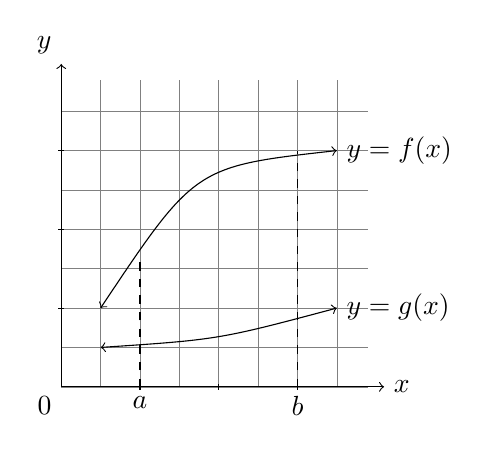
\begin{tikzpicture}[scale=1]
        \draw[step=0.5cm,gray,very thin] (0,0) grid (3.9,3.9);
        \draw[->] (0,0) -- (4.1,0);
        \draw[->] (0,0) -- (0,4.1);
        \node[anchor=south east] at (0,4.1) {$ y $};
        \node[anchor=west] at (4.1,0) {$ x $};
        \node[anchor=north east] at (0,0) {$ 0 $};
        \foreach \x in {1cm, 2cm, 3cm}
            \draw[] (\x,-1pt) -- (\x,1pt);
        \foreach \y in {1cm, 2cm, 3cm}
            \draw[] (-1pt,\y) -- (1pt,\y);

        \draw[<->] (0.5,1) .. controls (1.7,2.8) .. (3.5,3);
        \draw[<->] (0.5,0.5) .. controls (2,0.6) .. (3.5,1);
        \draw[dashed] (1,0) -- (1,1.6);
        \draw[dashed] (3,0) -- (3,3);
        \node[anchor=north] at (1,0) {$a$};
        \node[anchor=north] at (3,0) {$b$};
        \node[anchor = west] at (3.5,3) {$y=f(x)$};
        \node[anchor = west] at (3.5,1) {$y=g(x)$};
    \end{tikzpicture}
    \caption{Area between the lines}
    \label{Label}
\end{figure}
\begin{align*}
    Area &= \int_{a}^{b}f(x)\ dx - \int_{a}^{b}g(x)\ dx\\
    &= \int_{a}^{b}[f(x) - g(x)]\ dx
\end{align*}

\subsection{Example 1}
Find the area of the region bounded above by $y = e^x$, bounded below by $y = x$, and bounded on the sides by $x = 0$ and $x = 1$.
\begin{figure}[h]
    \centering
    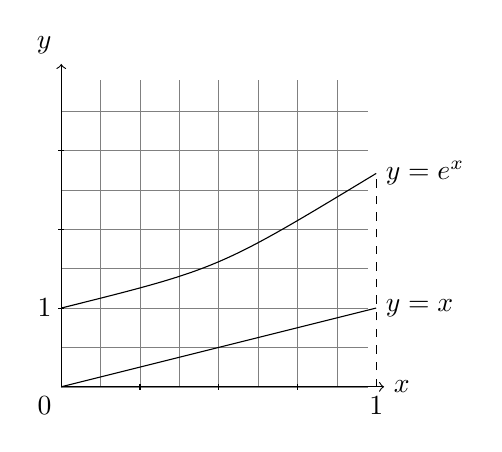
\begin{tikzpicture}[scale=1]
        \draw[step=0.5cm,gray,very thin] (0,0) grid (3.9,3.9);
        \draw[->] (0,0) -- (4.1,0);
        \draw[->] (0,0) -- (0,4.1);
        \node[anchor=south east] at (0,4.1) {$ y $};
        \node[anchor=west] at (4.1,0) {$ x $};
        \node[anchor=north east] at (0,0) {$ 0 $};
        \foreach \x in {1cm, 2cm, 3cm}
            \draw[] (\x,-1pt) -- (\x,1pt);
        \foreach \y in {1cm, 2cm, 3cm}
            \draw[] (-1pt,\y) -- (1pt,\y);

        \draw[] (0,1) .. controls (2,1.5) .. (4,2.71);
        \draw[] (0,0) -- (4,1);
        \node[anchor = north] at (4,0) {$1$};
        \node[anchor = east] at (0,1) {$1$};
        \node[anchor = west] at (4,2.71) {$y=e^x$};
        \node[anchor = west] at (4,1) {$y=x$};
        \draw[dashed] (4,0) -- (4,2.71);
    \end{tikzpicture}
    \caption{Caption}
    \label{Label}
\end{figure}
\begin{align*}
    A &= \int_{0}^{1}(e^x - x)\ dx
    = e^x - \frac{1}{2}x^2\bigg]_0^1\\
    &= \Big(e^1 - \frac{1}{2}1^2\Big) - \Big(e^0 - \frac{1}{2}0^2\Big)\\
    &= e^1 - \frac{1}{2} - 1 = e - \frac{3}{2}\ \text{units}^2
\end{align*}

\subsection{Example 2}
Find the area of the region enclosed by the parabolas $y = x^2$ and $y = 2x - x^2$.\\
\begin{figure}[h!]
    \centering
    
\includegraphics[scale=0.5]{fig_6_2.png}
    \caption{Example 2}
    \label{Label}
\end{figure}
\\[8pt]
First, we solve the two equations and find the interesections: $ (0,0) \text{ and } (1,1) $, so
\begin{align*}
    A &= \int_{0}^{1}[(2x-x^2) - (x^2)]\ dx
    = \int_{0}^{1}(2x-2x^2)\ dx\\
    &= 2\ \int_{0}^{1}(x-x^2)\ dx\\
    &= 2\ \Big[\frac{1}{2}x^2 - \frac{1}{3}x^3\Big]_0^1\\
    &= 2\ \bigg\{ \Big[ \frac{1}{2} (1)^2 - \frac{1}{3} (1)^3 \Big] - \Big[ \frac{1}{2} (0)^2 - \frac{1}{3} (0)^3 \Big] \bigg\}\\
    &= 2\Big( \frac{1}{6} \Big) = \frac{1}{3}\text{units}^2
\end{align*}

\subsection{Example 5}
Find the area of the region bounded by the curves $y = \sin x$, $y = \cos x$, $x = 0$, and $x = \pi / 2$ .
\begin{figure}[h]
    \centering
    
\includegraphics[scale=0.5]{fig_6_5.png}
    \caption{Example 5}
    \label{Label}
\end{figure}
\\[8pt]
The points of intersection occur when $ \sin x = \cos x $, that is, when $ x = \pi /4 $. Then the required area is:
\begin{align*}
    A &= \int_{0}^{\pi /2}|\cos x - \sin x|\ dx = A_1 + A_2\\
    &= \int_{0}^{\pi /4}(\cos x - \sin x)\ dx + \int_{\pi /4}^{\pi /2}(\sin x - \cos x)\ dx\\
    &= \big[ \sin x - \cos x \big]_0^{\pi /4} + \big[-\cos x + \sin x \big]_{\pi / 4}^{\pi /2}\\
    &= \bigg( \frac{1}{\sqrt{2}} + \frac{1}{\sqrt{2}} - 0 - 1 \bigg) + \bigg( -0-1 + \frac{1}{\sqrt{2}} + \frac{1}{\sqrt{2}} \bigg)\\
    &= 2 \sqrt{2} - 2
\end{align*}

\pagebreak
\subsection{Example 6 **On test do both ways}
Find the area enclosed by the line $ y=x-1 $ and the parabola $ y^2=2x+6 $.
\begin{figure}[h]
    \begin{subfigure}[h]{0.5\textwidth}
        \centering
        
\includegraphics[scale=0.5]{fig_6_6_1.png}
        \caption{Example 6}
        \label{Label}
    \end{subfigure}
    \begin{subfigure}[h]{0.5\textwidth}
        \centering
        
\includegraphics[scale=0.5]{fig_6_6_2.png}
        \caption{Example 6}
    \end{subfigure}
\end{figure}
\\[8pt]
\textbf{Method 1}
\begin{align*}
    \text{Area} = \int_{-3}^{1}\big[\sqrt{2x+6} - (-\sqrt{2x+6})\big] + \int_{-1}^{5}\big[\sqrt{2x+6} - (x-1)\big]\ dx
\end{align*}

\noindent
\textbf{Method 2}\\
We should look at the figure sideways, then $ y^2 = 2x+6 $ becomes $ x=(y^2-6)/2 $, $ y=x-1 $ becomes $ x=y+1 $. The intersections becomes $ (-1, -2) $ and $ (5,4) $.
\begin{align*}
    \text{Area} = \int_{-2}^{4}\bigg[ (y+1) - \bigg( \frac{y^2 - 6}{2} \bigg) \bigg]\ dy
\end{align*}

\end{document}
